\section{Theorie}
\label{sec:Theorie}
Unter dem Faraday-Effekt versteht man die Drehung der Polarisationsebene einer elektromagnetischen Welle in einem Medium durch den Einfluss eines Magnetfeldes, welches parallel zur Ausbreitungsrichtung dieser ist. \\
Außerdem ist es möglich Rückschlüsse auf die Bandstruktur des Testmediums zu ziehen.
\subsection{Effektive Masse}
\label{sec:effektive_masse}
Mit Hilfe der effektiven Masse ist es möglich die physikalischen Effekte der Bandstruktur eines Halbleiters approximiert zu beschreiben. In Abbildung \ref{fig:band} ist die Bandstruktur von Leitungs- bzw. Valenzband dargestellt.
\begin{figure}
  \centering
  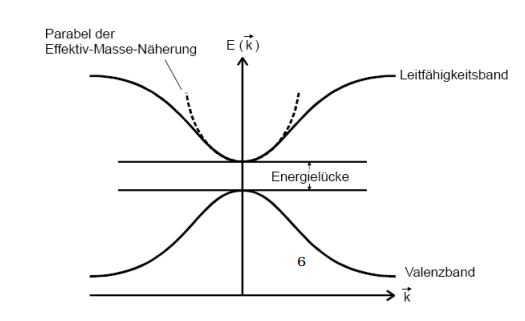
\includegraphics[scale=0.7]{fig/band.png}
  \caption{Vereinfachte Darstellung der Bandstruktur eines Festkörpers. \cite[6]{Bild2}}
  \label{fig:band}
\end{figure}
Um das Minimum herum wird die Energie des Bandes $\varepsilon$ in Abhängigkeit des Wellenzahlvektors $\vec{k}$ genähert. Dies geschieht mit Hilfe einer Taylorreihe:
\begin{equation}
  \label{eqn:energiegl}
  \varepsilon(\vec{k})=\varepsilon(0) + \frac{1}{2}\sum_{i=1}^3 \left.\frac{\partial^2 \varepsilon}{\partial k_i^2}\right|_{k=0}k_i^2 + \mathcal{O}(k^3)
\end{equation}
Als nächstes vergleicht man analog zu Newtons zweitem Axiom die Beschleunigung in einem elektrischen Feld $E$. Dafür ergibt sich quantemechanisch betrachtet für ein Kristall-Elektron (\ref{eqn:kris})
 und für ein freies Teilchen im Vakuum (\ref{eqn:frei}):
\begin{align}
  \label{eqn:kris}
  a=\dfrac{1}{\hbar^2}\dfrac{\partial^2 \varepsilon}{\partial k^2}\cdot qE \\
  \label{eqn:frei}
  a=\dfrac{1}{m_\mathrm{e}}\cdot qE
\end{align}
Dabei ist $k$ die Wellenzahl, $\hbar$ das reduzierte plancksche Wirkungsquantum, $q$ die Ladung des Elektrons und $\varepsilon(k)$ die Energie in Abhängigkeit von $k$.
Damit wird die effektive Masse wie folgt definiert:
\begin{equation}
  \label{eqn:effmass}
  m^{*}_i := \frac{\hbar^2}{\left.\frac{\partial^2 \varepsilon}{\partial k_i^2}\right|_{k=0}}
\end{equation}
Dank der Berücksichtigung der Periodizität des Kristallpotentials $V(\vec{r})$ in dem Ausdruck für die effektive Masse siehe Gleichung \ref{eqn:effmass} ist es möglich den Hamilton-Operator $\hat{H}$ der Kristallelektronen in den
eines freien Teilchens umzuschreiben. Aus
\begin{equation*}
  \hat{H}=\dfrac{\hbar^2}{2m_\mathrm{e}}\nabla^2+V(\vec{r})
\end{equation*}
wird mit Gleichung (\ref{eqn:effmass})
\begin{equation*}
  \hat{H}=\dfrac{\hbar^2}{2m^*}\nabla^2 .
\end{equation*}
\subsection{Zirkulare Doppelbrechung}
\label{sec:zirkulare_doppelbrechung}
In diesem Abschnitt der Theorie geht es um zirkulare Doppelbrechung. Darunter versteht man die Drehung der Polarisationsebene von linear polarisiertem Licht $E(z)$ bei Transmission durch einen Kristall.
Dies lässt sich durch die unterschiedlichen Phasengeschwindigkeiten der Phasengeschwindigkeiten im Kristall für rechts- bzw. linkszirkulares polarisiertes Licht $E_\mathrm{R}$, $E_\mathrm{L}$ erklärn. Mathematisch bedeutet das für
die Zusammensetzung des Lichtstrahls als Linearkombination:
\begin{equation}
  \label{eqn:zusammen}
  \vec{E}(z)=\dfrac{1}{2}(\vec{E}_\mathrm{R}(z)+\vec{E}_\mathrm{L}(z)) \, \mathrm{mit} \, k_\mathrm{L}\neq k_\mathrm{R}
\end{equation}
Die rechts- bzw. linkszirkularen Anteile sind wie folgt definiert:
\begin{align}
  \label{eqn:rechtslinks}
  \begin{aligned}
  \vec{E}_\text{R}(z) &= \left(E_0 \vec{x}_0 - \text{i}E_0\vec{y}_0\right)\exp\left(\text{i}{k}_\text{R}z\right)\\
  \vec{E}_\text{L}(z) &= \left(E_0 \vec{x}_0 + \text{i}E_0\vec{y}_0\right)\exp\left(\text{i}{k}_\text{L}z\right).
\end{aligned}
\end{align}
Um nun das austretende Licht zu beschreiben werden zunächst zwei Winkel $\Psi$ und $\vartheta$ eingeführt:
\begin{align}
  \label{eqn:winkel}
  \begin{aligned}
    \Psi&:=\frac{L}{2}(k_\text{R}+k_\text{L}) \\
    \vartheta &:= \frac{L}{2}(k_\text{R}-k_\text{L}) \overset{k_i=\frac{n_i\omega}{\text{c}_0}}{=} \frac{L\omega}{2\text{c}_0}\left(n_\text{R}-n_\text{L}\right)
\end{aligned}
\end{align}
Setzt man nun Gleichung (\ref{eqn:rechtslinks}) in Gleichung (\ref{eqn:zusammen}) ein ergibt sich für das austretende Licht der folgende Ausdruck:
\begin{equation*}
  \vec{E}(L)=E_0 \exp(\text{i}\Psi)\left(\cos(\vartheta) \vec{x}_0 + \sin(\vartheta)\vec{y}_0\right)
\end{equation*}
Der Effekt ist schematisch in Abbildung (\ref{fig:brechung}) dargestellt.
\begin{figure}[h]
  \centering
  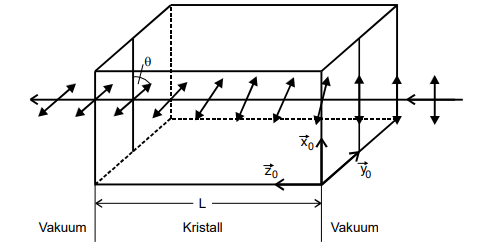
\includegraphics[scale=0.7]{fig/brechung.png}
  \caption{Darstellung von zirkularer Doppelbrechung bei Transmission eines Kristalls. \cite[1]{Anleitung}}
  \label{fig:brechung}
\end{figure}\\
\\
Die Entstehung dieses Effektes beruht auf den elektrischen Dipolmomenten die im Kristall erzeugt werden können. Diese induzierten Dipole erzeugen die Polarisation $\vec{P}$ des Kristalles. Diese ist unter der Vorraussetzung eines kleinen elektrischen Feldes $\vec{E}$ proportional zu diesem. Es gilt die Beziehung:
\begin{equation}
  \vec{P}=\varepsilon_\mathrm{0} \chi \vec{E}
\end{equation}
